\documentclass[a6paper, parskip=half, DIV=14, 12pt]{scrartcl}

\usepackage{galaofthegods}

\usepackage{mnemonic}

\color{greekbrown}
\begin{document}
{%
\thispagestyle{empty}
		\enlargethispage{3.5\baselineskip} % Move the bottom line (author and date) down a bit
\setmainfont[Scale=1.0]{URW Classico}
\begin{center}
%\makeatletter
%{\footnotesize Version \@version}
%\makeatother

%\vfill

{
\setmainfont[Scale=1.75]{URW Classico-Bold}
\Huge
The Trial of\\[0.5ex]Mnemosyne
%Mnemonic
}

\vfill

\begin{tikzpicture}
\node[draw, line width=2mm, greekbrown, fill=ForestGreen, inner sep=0pt, minimum height=8cm, minimum width=8cm, rounded corners=0.125in] at (0,0) {};
\node at (0,0) {
\includegraphics[height=6cm]{Images/brown_circle_frame}};
\node[inner sep=0pt] {
\includegraphics[height=7cm]{Images/themis.png}};
\end{tikzpicture}
%\tikz{\node[inner sep=0pt, xscale=-1] {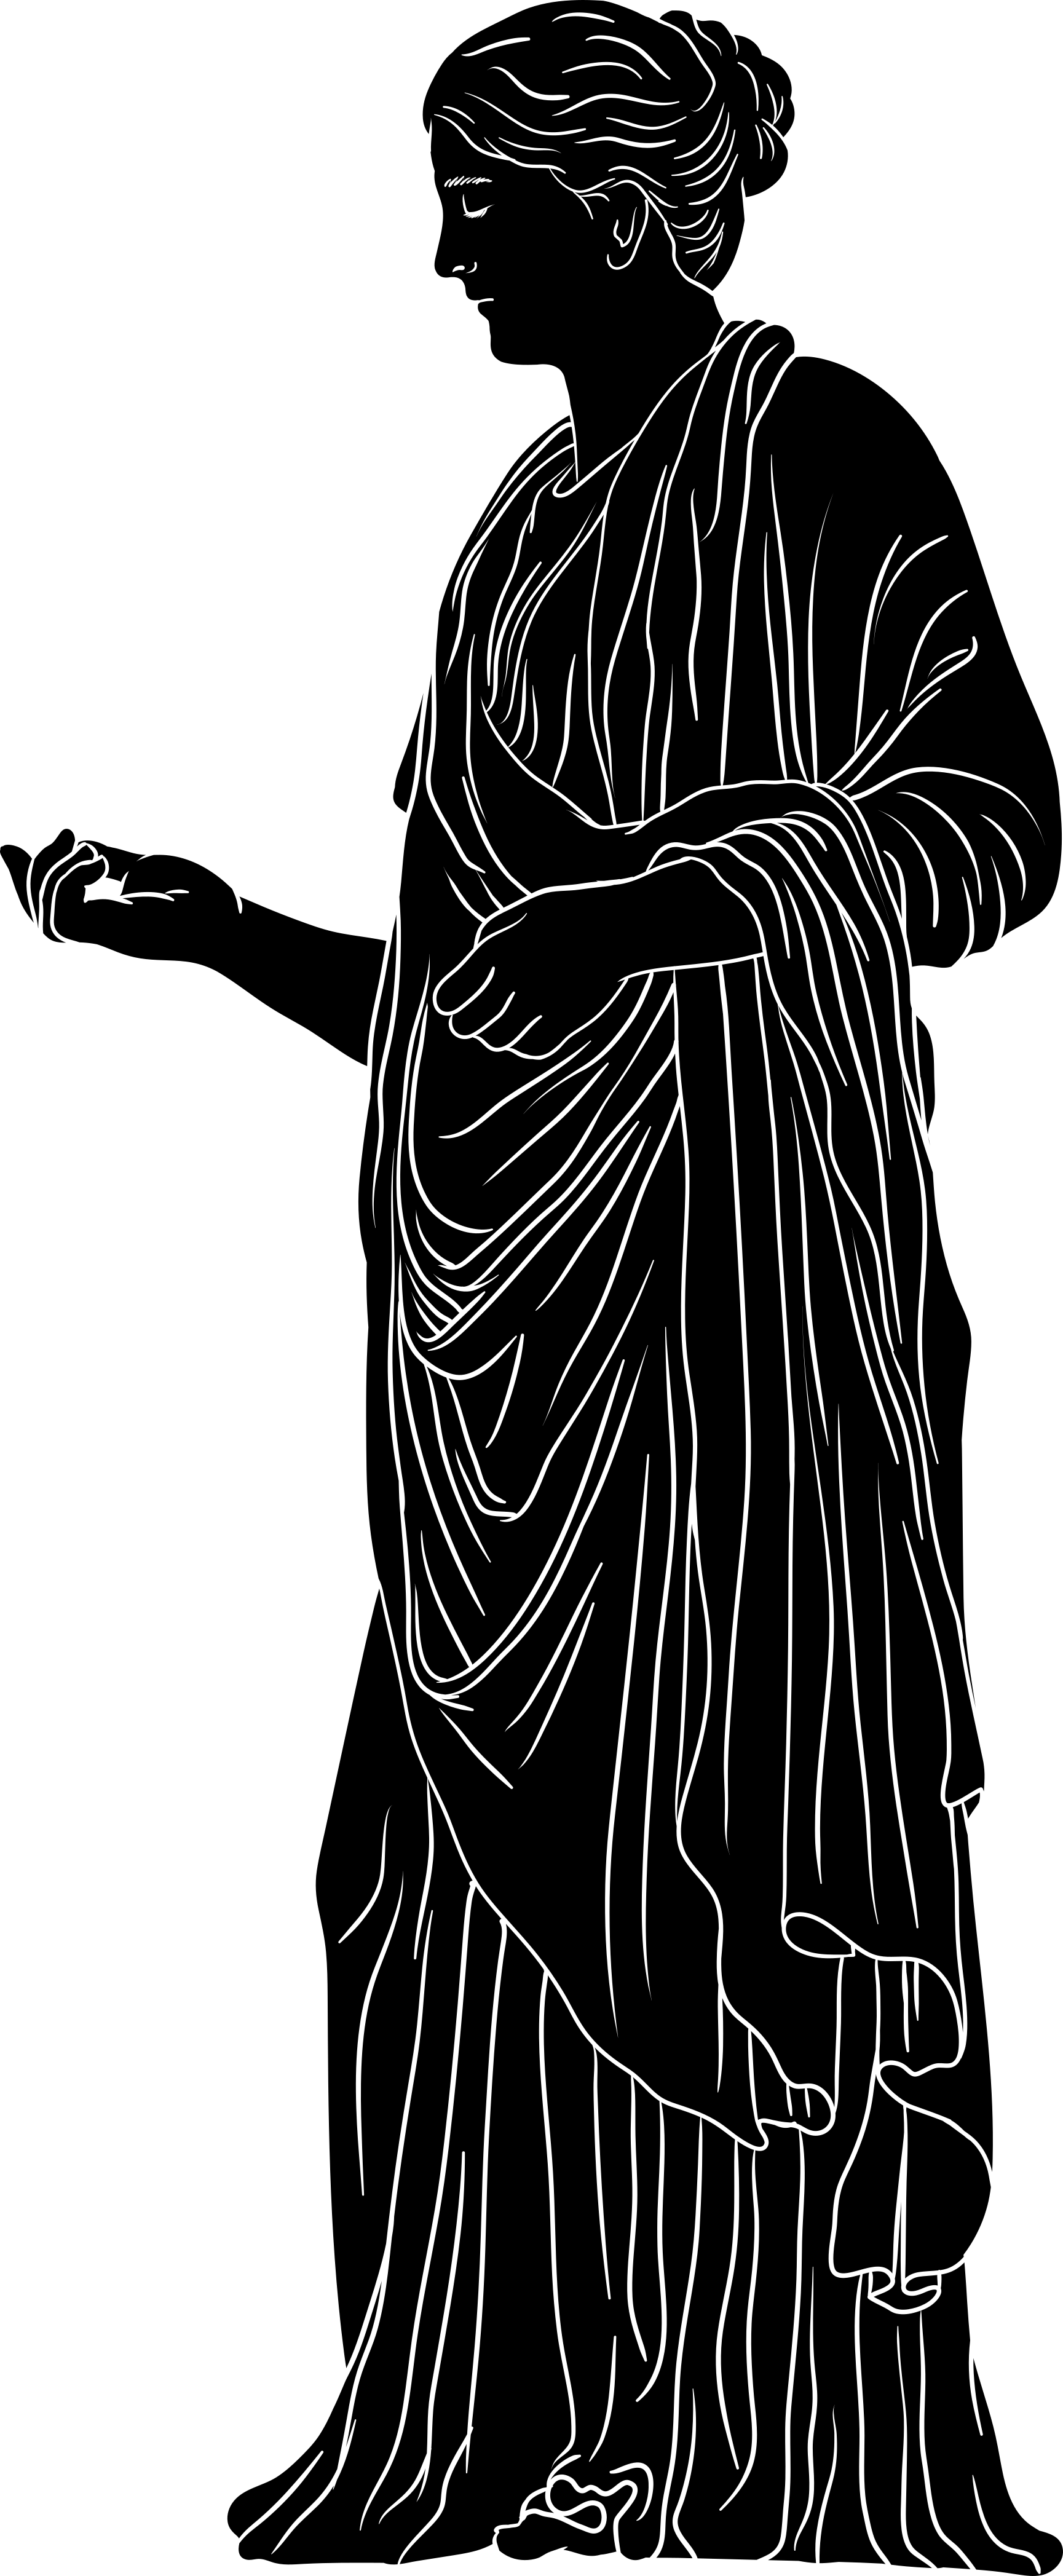
\includegraphics[height=7cm]{Images/statue_woman.png}};}
%\quad
%\tikz{\node[inner sep=0pt] {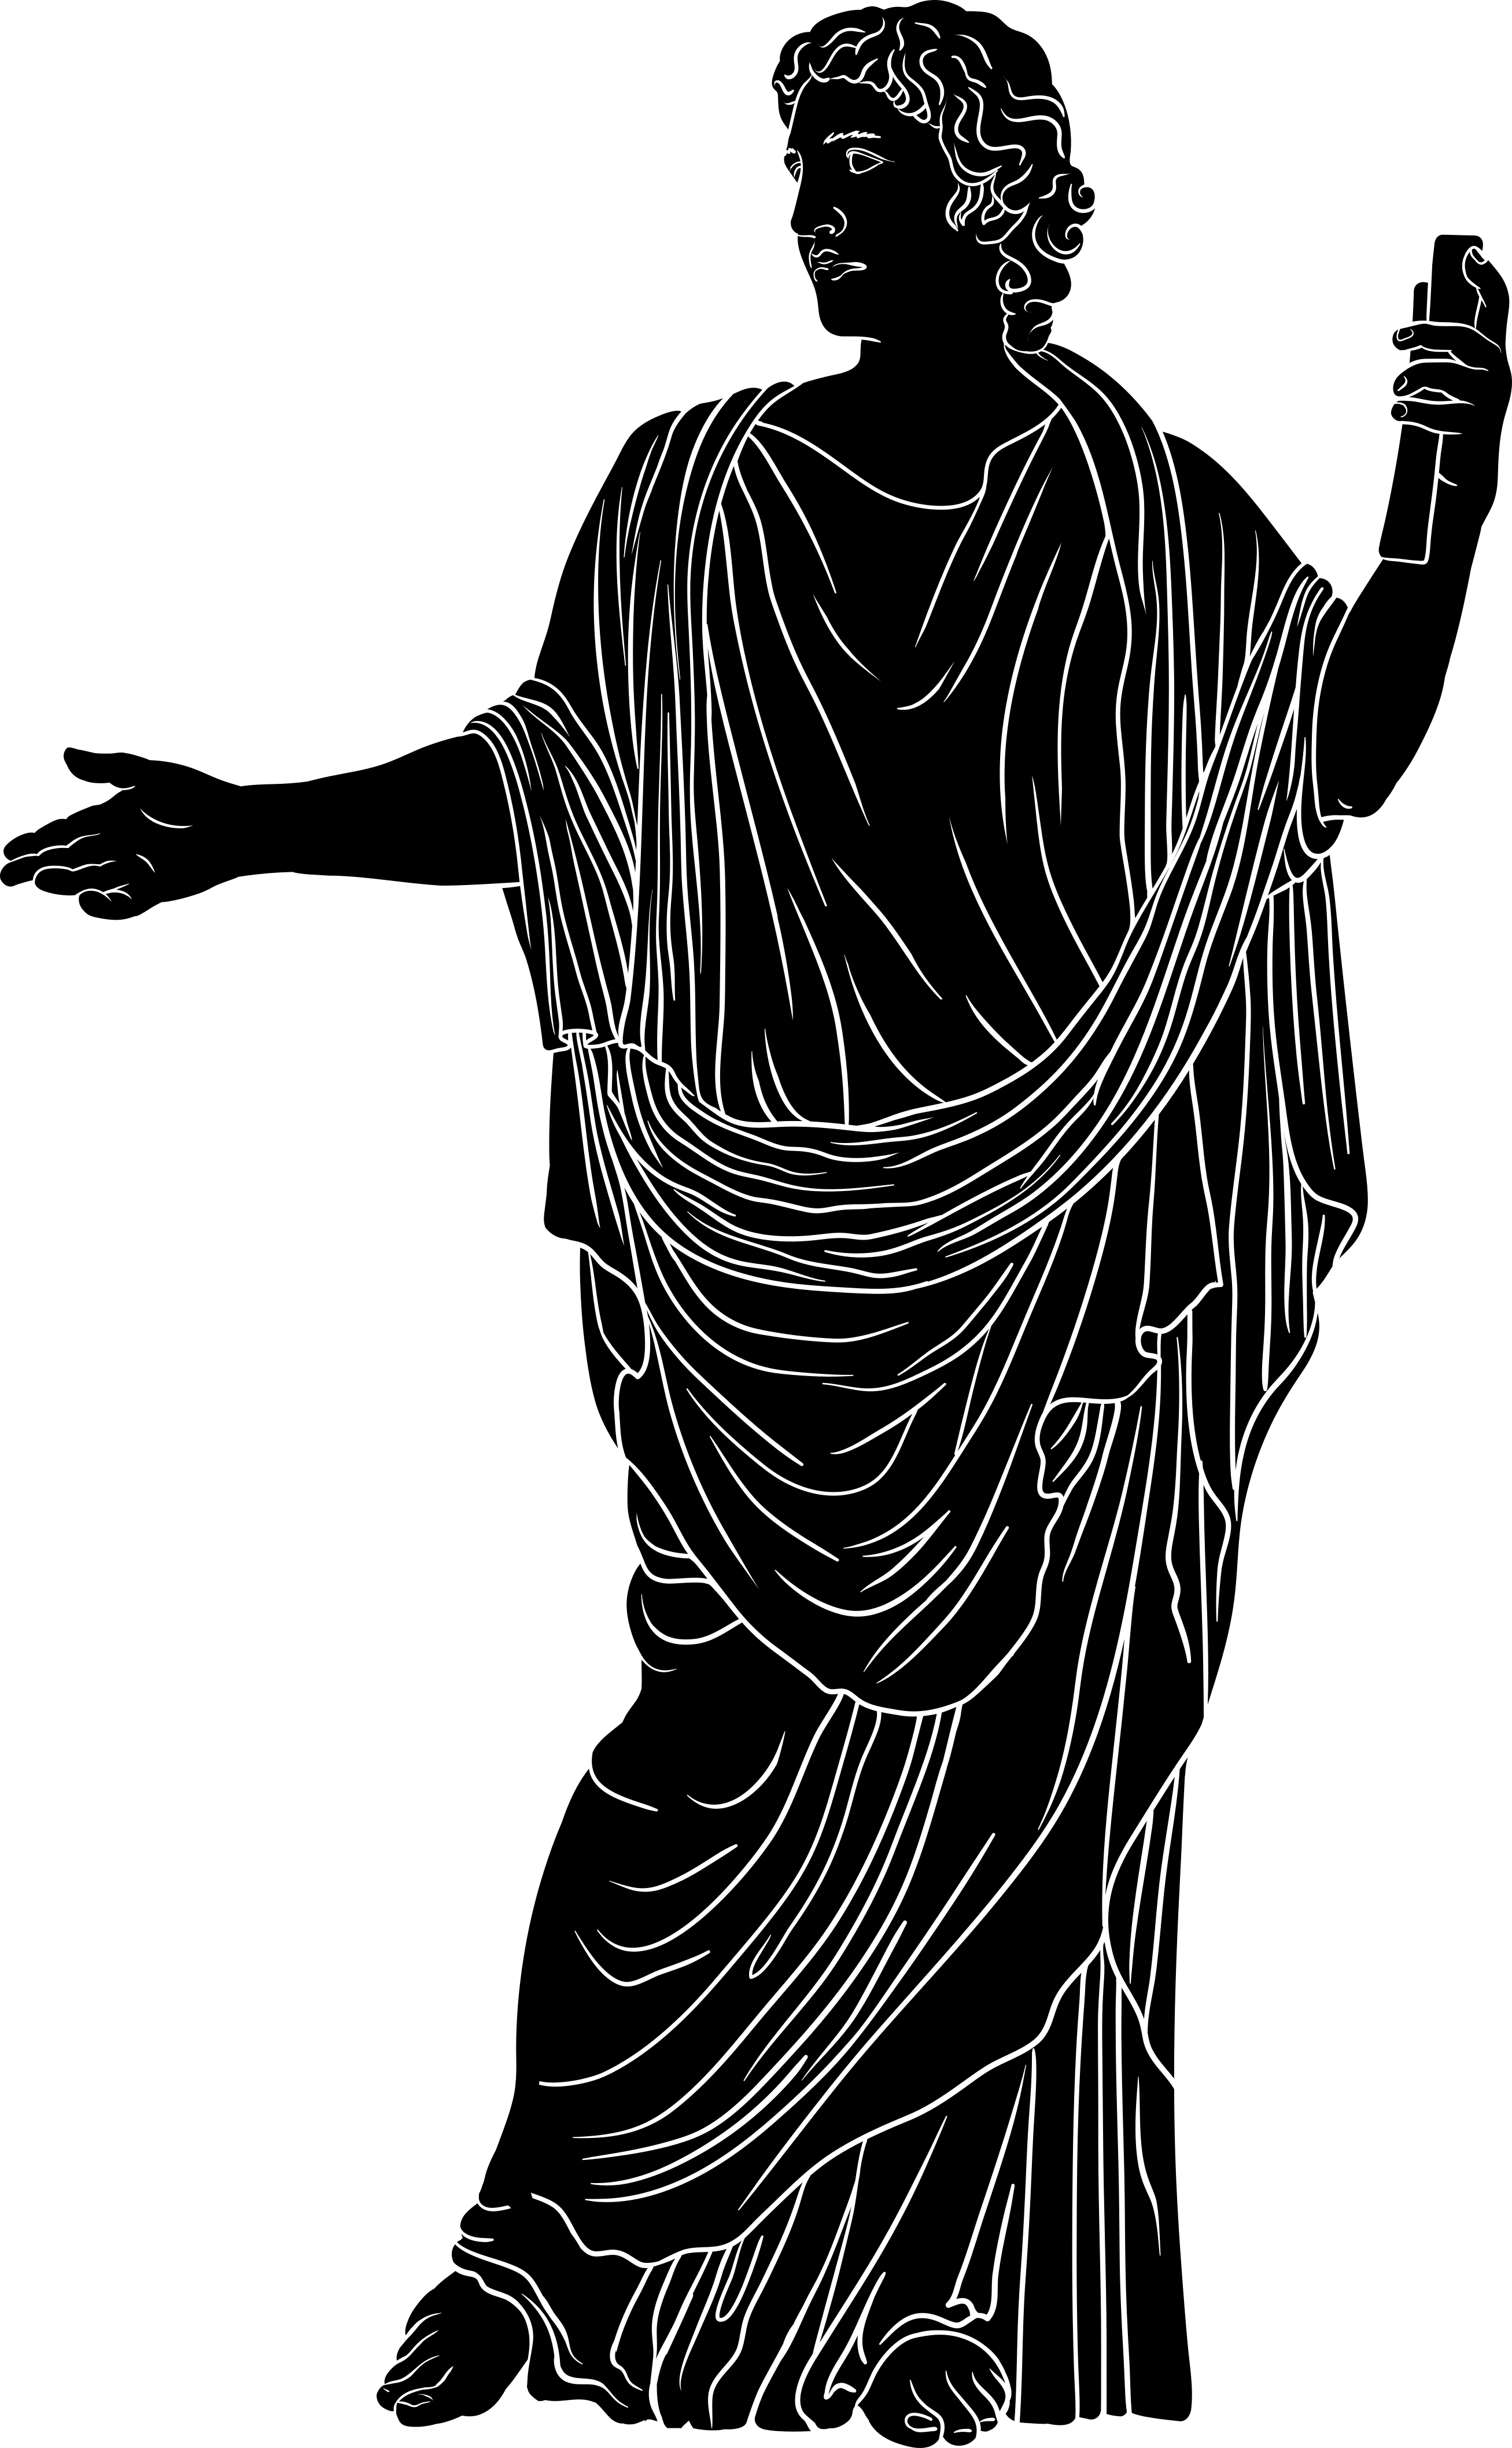
\includegraphics[height=7cm]{Images/statue_man.png}};}

\vfill{}

{
\setmainfont{URW Classico}
\large
Designed by Michael Purcell
}
\end{center}
}

\newpage
\section*{Overview}

The Trial of Mnemosyne is a cooperative storytelling and memory game for one or more players that can be played in about twenty minutes.

As you play, you will arrange a set of twenty-one cards in a crossword-style grid.
Your task is to memorize where each card is located in this grid.

To make this easier, you will invent a story about the cards as you arrange them.
Each card depicts a god or goddess from Greek mythology.
You will use the domains and personality traits of these familiar characters to inform the story that you create.

After you complete the grid, you will collect the cards, shuffle them, and then \textemdash{} using your story as a mnemonic \textemdash{} try to reconstruct the grid from memory.



\newpage

%\section*{Components}

\begin{itemize}[leftmargin=*]
\item 22 deity cards.
\end{itemize}

\section*{Setup}

\begin{enumerate}[leftmargin=*]
\item Shuffle the cards and place the shuffled deck face down on the table.
\item Draw one card and place it face up in the center of the play area. This first card is called the \emph{hero card}.
\item Decide who the hero of your story will be.
\begin{itemize}[leftmargin=*]
\item Use the domain or personality traits of the deity that is depicted on the hero card to inform your choice.
\item This hero can be anyone! They do not need to be an existing character from Greek mythology.% You can tell any kind of story that you want. Do whatever will best help you memorize how the cards are arranged.
\end{itemize}
\item Flip the hero card so that it is face down.

\end{enumerate}

\newpage

\section*{Gameplay}

The game consists of two phases, memorization and recitation.

During the memorization phase, you will arrange the deity cards in a crossword-style grid and tell a story to help you remember where each card is placed.

During the recitation phase, you will test your ability to use the story you told to recreate your arrangement.

%\newpage

\subsection*{Memorization}

The memorization phase consists of ten rounds.
During each round you will add two cards to the grid.
As you do you will augment your story to remind you of what cards you added and where you placed them.

Your story does not need to be a myth!
Choose whatever will help you remember how the deity cards are arranged.


\newpage

Each round you will:
\begin{enumerate}[leftmargin=*]
\item Draw two cards from the deck.
\item Decide where to place these new cards.
\begin{itemize}[leftmargin=*]
%	\item The two new cards must be placed so that they are adjacent to one another.
	\item The first new card must be placed adjacent to exactly one \emph{linking card} that is already in the grid.
	\item The second new card must be placed adjacent to the first new card, immediately opposite the linking card, and adjacent to no other cards.
%	\begin{itemize}[leftmargin=*]
%	\item adjacent to the first new card,
%	\item adjacent to no other cards,
%	\item so that it forms a straight line with the first new card and the linking card.
%	\end{itemize}
\end{itemize}
\item Extend your story to help you remember where these new cards are placed.
\begin{itemize}[leftmargin=*]
\item Use the domains and personality characteristics of the deities depicted on the cards to inform your story choices.
\item Use the linking card to connect this new story to what has come before.
\end{itemize}
\item Place the new cards in the grid and then flip them so that they are face down.
\end{enumerate}

\newpage

\subsection*{Recitation}

During the recitation phase you will try to reconstruct the grid you created during the memorization phase. To do so:
\begin{enumerate}[leftmargin=*]
\item Gather up all of the cards and shuffle them.
\item Spread the cards out face up on the table.
\item Locate the hero card (the first card you drew during setup) and place it in the middle of the play area.
\item Retell your story, finding and placing deity cards in the grid as you go.
\end{enumerate}

You win if, after finishing your story and placing all twenty-one cards in the grid, everyone agrees that you have correctly recreated your arrangement.

For an additional challenge, take a break before playing the recitation phase.
Can you recreate your arrangement if you wait for a day (or more) between phases?





\newpage

\section*{Example}

After shuffling the deck, Mike draws \emph{Poseidon} as his hero card.
Inspired by Poseidon's role as God of the Sea, Mike decides that his story will be about Carl the fisherman.

Mike draws \emph{Ares} and \emph{Hera} as his first pair of new cards.
He decides that the story these cards suggest is that Carl the fisherman got into a fight with his sister, Wanda. 

So, he places these two new cards in the grid with \emph{Ares} between \emph{Poseidon} and \emph{Hera}.
\begin{center}
\begin{tikzpicture}
\pic[xscale=0.25, yscale=0.25, transform shape] at (-\horizdist*0.25  - 0.0625in, 0) {character_card_front_alt_small={Poseidon}{poseidon_alt.png}{God of the Sea}{0.25in}{0.0in}{ForestGreen}{gray}{white}};
\pic[xscale=0.25, yscale=0.25, transform shape] at (0,0) {character_card_front_alt_small={Ares}{ares.png}{God of War}{0.0in}{-0.125in}{CornflowerBlue}{gray}{white}};
\pic[xscale=0.25, yscale=0.25, transform shape] at (\horizdist*0.25 + 0.0625in, 0) {character_card_front_alt_small={Hera}{hera_alt.png}{Goddess of Family}{0.0in}{0.125in}{CornflowerBlue}{gold}{white}};
\end{tikzpicture}
\end{center}
\textbf{Note:} These cards are shown face up here in the interest of clarity. In a real game, however, all cards are played face down.

\newpage

Mike then draws \emph{Zeus} and \emph{Hecate}.
He decides that, after their fight, Carl and Wanda saw a spectacular cloud formation which revealed a prophecy about their future.

So, he places these two new cards in the grid with \emph{Zeus} between \emph{Ares} and \emph{Hecate}.

\begin{center}
\begin{tikzpicture}
\pic[xscale=0.25, yscale=0.25, transform shape, rotate=90] at (0, -\horizdist*0.25  - 0.0625in) {character_card_front_alt_small={Poseidon}{poseidon_alt.png}{God of the Sea}{0.25in}{0.0in}{ForestGreen}{gray}{white}};
\pic[xscale=0.25, yscale=0.25, transform shape, rotate=90] at (0,0) {character_card_front_alt_small={Ares}{ares.png}{God of War}{0.0in}{-0.125in}{CornflowerBlue}{gray}{white}};
\pic[xscale=0.25, yscale=0.25, transform shape, rotate=90] at (0, \horizdist*0.25 + 0.0625in) {character_card_front_alt_small={Hera}{hera_alt.png}{Goddess of Family}{0.0in}{0.125in}{CornflowerBlue}{gold}{white}};

\pic[xscale=0.25, yscale=0.25, transform shape, rotate=90] at (\vertdist*0.25 + 0.0625in, 0) {character_card_front_alt_small={Zeus}{zeus.png}{God of the Sky}{0.125in}{0.0in}{CornflowerBlue}{brown}{white}};
\pic[xscale=0.25, yscale=0.25, transform shape, rotate=90] at (2\vertdist*0.25 + 0.125in, 0) {character_card_front_alt_small={Hecate}{hecate.png}{Goddess of Prophecy}{0.0in}{0.03in}{Purple}{gray}{white}};

\end{tikzpicture}
\end{center}


\vfill

\hrulefill

{\footnotesize \textbf{Design}: Michael Purcell \hfill \textbf{Contact}:~\href{mailto:mike@armiger.games}{mike@armiger.games}}

\end{document}
